\section{Model}
We propose a deep reasoning model (DRM) with an architecture as shown in Figure \ref{fig:systemDiagram}. The model has three components: the state generation module (SGM) implemented with two convolutional neural networks; the reasoning generation module (RGM) implemented as deep reinforcement learning via an actor-critic algorithm; and a context selection operator (CSO) that shrinks the text context given a discourse marker and a direction (left=before; right=after).

% We present model component details in Section \ref{sec2description} and the design intuitions in Section \ref{sec2intuition}.



\begin{figure}
\begin{minipage}{.45\textwidth}
 \centering
 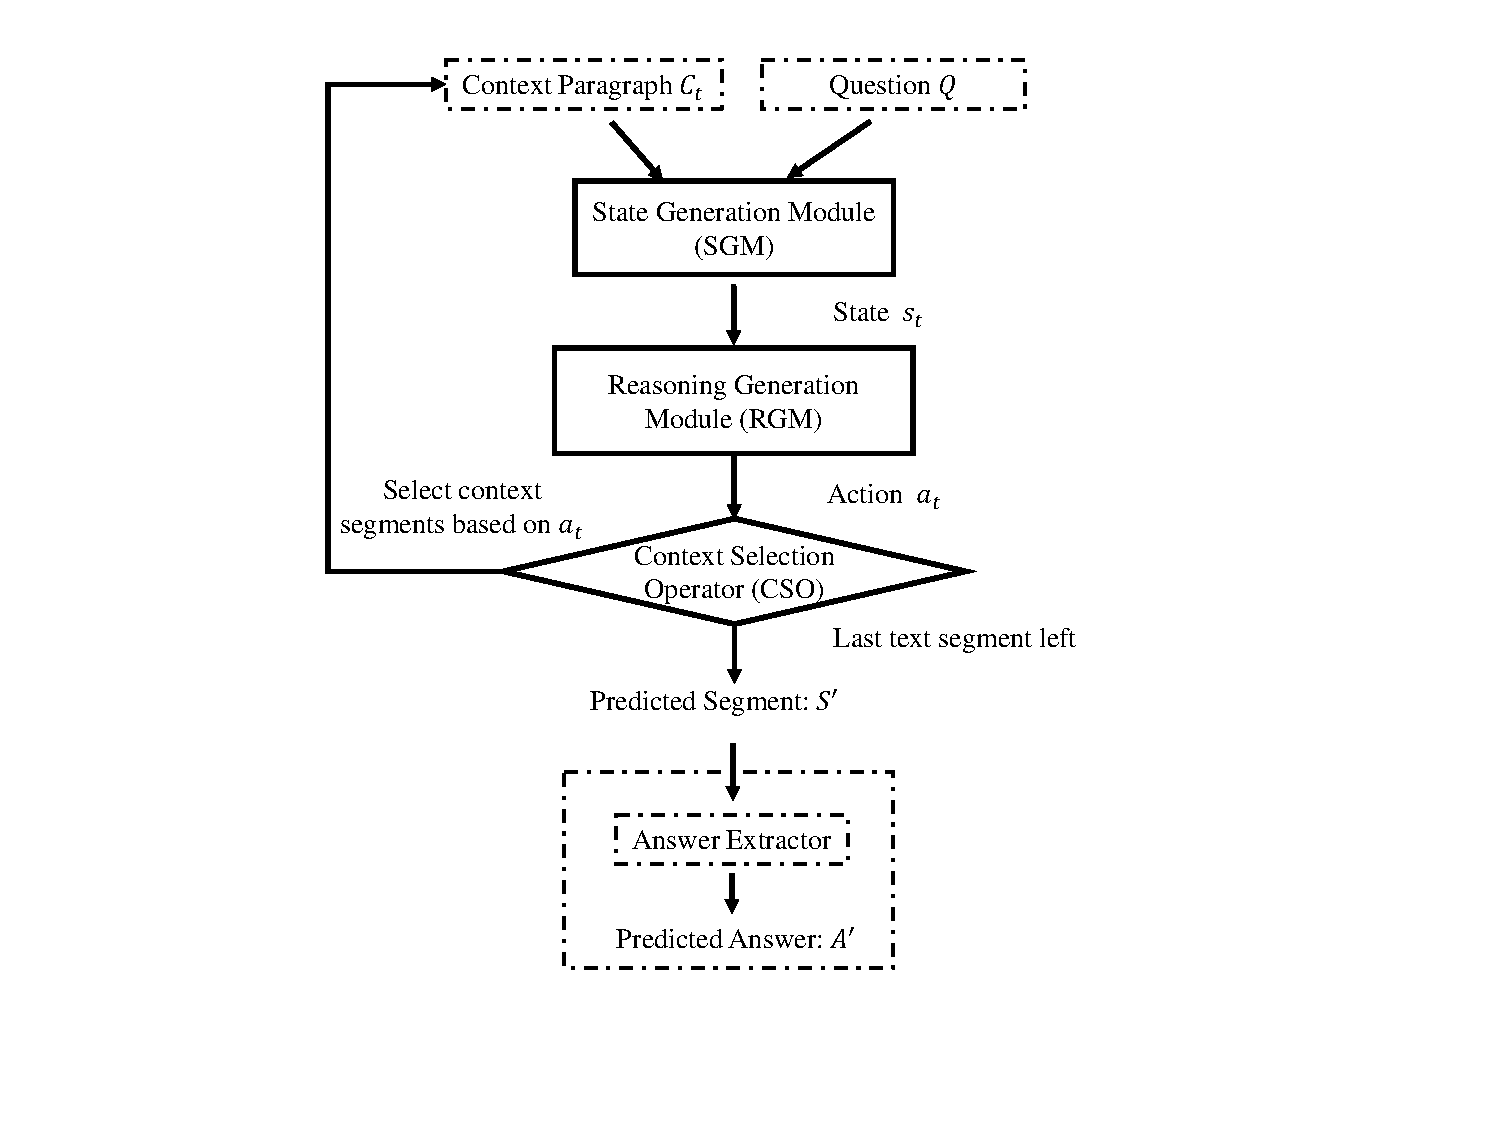
\includegraphics[width=0.9\linewidth]{fig/fig1.pdf}
 \caption{System Diagram}
 \label{fig:systemDiagram}
\end{minipage}
\vspace{-2ex}
\end{figure}
%[Yu] \kechen{basic idea of RL and insight of using RL, multi step decision is naturally modeled by MDP}
% \subsection{Model Component Overview}
\label{sec2description}
The goal of our system is to mimic human reading behavior to extract a segment that
contains the answer. The mechanic in reducing the text context is analogous to binary search: Let $D=(D^1,D^2,...,D^k)$ be a list of discourse markers that appears in a context paragraph $C$. These discourse markers, working as the candidate partition points, divide the context into a list of segments $S=(S^1,S^2,...,S^{k+1})$. Then the context can be represented by a mixture of discourse markers and segments, $C=(S^1, D^1, S^2, D^2,...,D^k, S^{k+1})$. To identify the correct segment $S^*$ from $S$, our model at time-step $t$ works as follows:\\
(a) SGM encodes the context $C_t$ and question $Q$ into a vector representation, \emph{i.e.} the state $s_t$.\\
(b) RGM takes the state $s_t$ as its input, and predicts the partition point $D^{p(s_t)}_t$ (${p(s_t)}$ is the index selected at \emph{t}) and the reading focus $f_t \in \{left, right\}$. An action is defined as $a_t=(D^{p(s_t)}_t,f_t)$. \\
(c) CSO divides $C_t$ into two parts from $D^{p(s_t)}_t$: $C^1_t=(S^1, D^1,...,D^{p(s_t)-1}, S^{p(s_t)})$ and $C^2_t=(S^{p(s_t)+1}, D^{p(s_t)+1},...,D^k, S^{k+1})$, and keeps $C_{t+1} \leftarrow C_{t}^{1}$ if $f_t$ is left or $C_{t+1} \leftarrow C_{t}^{2}$ if $f_t$ is right. \\
The iterations stop when the output only contains a single text segment enclosed by two neighbor discourse markers. Intermediate output $D^{p(s_t)}_t$ at each time-step constitutes a reasoning path $(D^{p(1)}_1,...,D^{p(s_t)}_t)$. We note that during the prediction procedure the context $C_t$ changes, while the question $Q$ not. \kechen{The process is summarized in Algorithm \ref{alg:train_beam}.}

% \emph{Remarks:}
It is possible to add an answer extractor following the text segment $S'$ for a final answer (dashed in Figure \ref{fig:systemDiagram}). Since this is not our paper's focus and many existing works have been done achieve decent performance \cite{DBLP:conf/ijcai/HuPHQW018}, so this module is not discussed in this paper. %\cite{DBLP:conf/acl/WangYWCZ17,DBLP:journals/corr/abs-1804-09541,DBLP:conf/ijcai/HuPHQW018}. Since this is not our paper's focus, we do not discuss it here.\\


%Since our paper's focus is not on answer extraction, and many existing works have been done achieve decent performance \cite{DBLP:conf/acl/WangYWCZ17,DBLP:journals/corr/abs-1804-09541,DBLP:conf/ijcai/HuPHQW018}, so this module is not discussed in this paper.



\begin{algorithm}
\fontsize{9}{10}\selectfont
  \SetKwInOut{Input}{Input}
  \SetKwInOut{Output}{Output}

 % \underline{function Euclid} $(a,b)$\;
  \Input{$C$: context, $Q$: question}
  \Output{Answer segment: a single text segment enclosed by two neighbor discourse markers}
  $t = 0$\\
  $C_0 \leftarrow C$\\
  % Initialize model parameters\\
  \While {$C_t$ contains more than one text segment}{
    %SGM encodes the context $C_t$ and question $Q$ into a vector representation $s_t$.\\
    $s_t = SGM(C_t, Q)$ // generate state\\
    $D^{p(s_t)}_t,f_t= RGM(s_t)$ // generate action\\ 
   % $a_t=(D^{p(s_t)}_t,f_t)$ // an action consists of partition point $D^{p(s_t)}$ and reading focus $f_t$\\
    $C^1_t, C^2_t = CSO(C_t, D^{p(s_t)}_t)$\\
    \uIf{$f_t==left$}{
    //$C^1_t=(S^1, D^1,...,D^{p(s_t)-1}, S^{p(s_t)})$\\
        $C_{t+1} \leftarrow C_{t}^{1}$ 
    }\Else{
    //$C^2_t=(S^{p(s_t)+1}, D^{p(s_t)+1},...,D^k, S^{k+1})$\\
        $C_{t+1} \leftarrow C_{t}^{2}$ 
    }
    $t = t + 1$
  }
  $S^* \leftarrow C_t$\\
  \Return{$S^*$}
  \caption{Identifying the correct answer segment from the context}
	  \vspace{-1ex}
  \label{alg:train_beam}
\end{algorithm}
\subsection{Deep Reinforcement Learning}\label{sec2intuition}
%As described in the introduction, in order to build a "smart" machine comprehension system by imitating a human-like reasoning process, we leverage a deep reinforcement learning (DRL) based structure to infer the reasoning steps guided by the discourse markers and/or the target words. There are two main reasons to choose DRL as our fundamental model structure:\\

We leverage a deep reinforcement learning (DRL) based structure to implement the system introduced in the above section. 
For every given context-question pair, the dataset provides an answer. Although this answer can be used to evaluate the final output of any reasoning path, there is no ground truth to evaluate the performance of each intermediate reasoning step $D^{p(s_t)}_t$. There are usually several different reasoning paths leading to the correct answer segment, based on different sequences of selecting discourse markers; thus the  task of searching for the best path fits well into the reinforcement learning, as these actions can reasonably imitate the human actions.
% , which makes our model more interpretable.
% It enables a flexible number of action steps to gradually search for the correct answer instead of generating the answer from end-to-end.
%There are also many possible reasoning paths which can lead to the same correct answer. In order to search such a reasoning path, %, just like searching for one possible route in a maze, DRL based approaches are very suitable. 

%2.  \kechen{merge 1 and 2? introduce reasoning path?}

A typical reinforcement learning structure contains four main elements: the state ($s_t$), the action ($a_t$), the reward ($r_t$), and the policy ($\pi$). In general, by taking an action $a_t$, a RL agent can move from its current state $s_t$ to another state $s_{t+1}$ and receive a reward $r_t$. The final target of a RL model is to learn an optimal policy $\pi$ such that the system can maximize the expected total reward $R_t=\mathop{\mathbb{E}}_\pi[\sum_{t=0}^{T}\gamma^t r_t]$ obtained at each state $s_t$, where $s_T$ is the final state. Specifically in our problem, at each time-step $t$ our model is in state $s_t$ containing the information of the current context $C_t$ and the question $Q$; it takes action $a_t$ choosing the appropriate discourse marker and the direction (reading focus) in order
to maximize the expected reward $R_t$. 
%*This expected reward can be further interpreted as the probability of finding the final correct answer by choosing this discourse marker and its reading direction.

%\cheng{unclear}